\documentclass[11pt]{article}
\usepackage[T1]{fontenc}
\usepackage{lmodern,microtype}
\usepackage[margin=1in]{geometry}
\usepackage{amsmath,amssymb,amsthm,mathtools}
\usepackage{booktabs,array,enumitem,tikz,xcolor,url}
\usetikzlibrary{arrows.meta,positioning}
\usepackage[colorlinks=true,linkcolor=blue!55!black,citecolor=green!35!black,urlcolor=blue!55!black]{hyperref}
\usepackage[nameinlink,noabbrev]{cleveref}

\setlist{nosep}
\setlength{\parskip}{0.35em}
\setlength{\parindent}{0pt}
\setlength{\emergencystretch}{2em}

\newtheorem{theorem}{Theorem}[section]
\newtheorem{proposition}[theorem]{Proposition}
\newtheorem{lemma}[theorem]{Lemma}
\newtheorem{corollary}[theorem]{Corollary}
\newtheorem{definition}[theorem]{Definition}
\theoremstyle{remark}
\newtheorem{remark}[theorem]{Remark}

\newcommand{\Ztwo}{\mathbb Z_2}
\newcommand{\C}{\mathbb C}
\newcommand{\R}{\mathbb R}
\newcommand{\M}{\mathcal M}
\newcommand{\V}{\mathcal V}
\newcommand{\TCr}{R_{\mathrm{TC}}}
\newcommand{\TCw}{W_{\mathrm{TC}}}
\newcommand{\TCs}{S_{\mathrm{TC}}}
\newcommand{\JC}{\mathrm{JC}}
\newcommand{\Tmove}{\mathsf T}
\newcommand{\xor}{\mathbin\oplus}
\newcommand{\whp}{\widehat p}

\definecolor{retic}{RGB}{176,43,43}
\definecolor{treecol}{RGB}{37,85,155}
\tikzset{
  vertex/.style={circle,draw,minimum size=5.5mm,inner sep=1pt,fill=white},
  treev/.style={vertex,draw=treecol,thick},
  reticv/.style={vertex,draw=retic,thick,double},
  leaf/.style={circle,draw,minimum size=4.8mm,inner sep=.4pt,fill=white},
  ordinary/.style={line width=.7pt},
  reticedge/.style={-{Stealth[length=2mm]},draw=retic,line width=.85pt}
}

\hypersetup{
  pdftitle={Full-Dimensional Jukes--Cantor Ambiguity in Weakly Tree-Child Level-2 Networks},
  pdfauthor={Alec Kriebel},
  pdfsubject={Phylogenetic-network identifiability under the Jukes--Cantor model},
  pdfkeywords={phylogenetic networks, Jukes--Cantor, identifiability, level 2, tree-child}
}

\title{Full-Dimensional Jukes--Cantor Ambiguity in\\
Weakly Tree-Child Level-2 Networks\\
\large An exact four-leaf construction and an all-taxa extension}
\author{Alec Kriebel\\\small Independent Researcher}
\date{August 2026}

\begin{document}
\maketitle

\begin{abstract}
We give two explicit four-leaf binary level-2 semi-directed phylogenetic
networks whose labelled mixed graphs are nonisomorphic and cannot be related
by redirecting their unique triangle, but whose open Jukes--Cantor model
images share a regular relatively open subset of full dimension eight.  Each
network has a tree-child rooting, but neither is strongly tree-child in the
semi-directed sense that every admissible rooting is tree-child.  The proof is
exact: on the physical locus, both models lie on the same irreducible
eight-dimensional component cut out by six Fourier equations; an algebraic
common point lies
strictly inside the positive-definite stochastic parameter space; and
rank-eight Jacobian minors are nonzero on both parameterizations.  An
independent verifier checks all 256 Fourier coordinates in a quadratic number
field.  Replacing corresponding leaves by identical rooted binary trees has
a positive analytic inverse.  Consequently, for every $n\ge4$ there is such
a non-triangle ambiguity on $n$ leaves, with a common regular open region of
dimension $2n$.  The result supplies an exact negative instance among
same-type four-leaf level-2 comparisons and gives a precise obstruction to extending
identifiability statements from strongly to merely weakly tree-child
semi-directed networks.
\end{abstract}

\noindent\textbf{Keywords.} phylogenetic networks; identifiability;
Jukes--Cantor model; level-2 networks; tree-child networks; algebraic
statistics.

\medskip
\noindent\textbf{MSC 2020.} 92B10, 62R01, 14P10, 05C05.

\section{Introduction}

A phylogenetic-network topology is scientifically recoverable from exact
site-pattern data only when distinct topologies cannot generate the same
generic distribution.  For trees this question has a long algebraic history;
for networks, mixtures over displayed trees introduce additional
nonidentifiability.  Triangle orientation is one familiar source: under
group-based models, redirecting the reticulation inside a small triangle can
preserve a full-dimensional part of the model.

This paper exhibits a different phenomenon at level two.  The two networks
have the same unlabelled theta core, but exchange two labelled pendant
components between a vertex on the unique triangle and a vertex off that
triangle.  Their standard semi-directed graphs are therefore not related by
triangle redirection.  Nevertheless, their Jukes--Cantor (JC) images meet in
full dimension on the open stochastic parameter space.

The tree-child convention is essential.  Following the semi-directed
terminology of Holtgrefe et al.~\cite{HoltgrefeEtAl2026}, a semi-directed
topology is \emph{weakly tree-child} if it has at least one tree-child rooting
and \emph{strongly tree-child} if every admissible rooting is tree-child.  The
pair below is weakly but not strongly tree-child.  It therefore does not
contradict the triangle-free strongly tree-child identifiability theorem of
Englander et al.~\cite{EnglanderEtAl2026}; instead it shows that allowing all
weakly tree-child topologies introduces a genuinely non-triangle ambiguity.

Ardiyansyah~\cite{Ardiyansyah2021} classified several four-leaf simple
level-2 comparisons algebraically and identified same-type comparisons that
were not resolved by those calculations.  The construction below supplies an
exact negative instance for one labelled pair of the triangle-containing
type.
It is distinct from the three-leaf semialgebraic triangle-orientation overlap
studied by Currie et al.~\cite{CurrieEtAl2026}, and from the stacked-
reticulation and two-blob local modifications studied by
Sullivant~\cite{Sullivant2026}.  Brits et al.~\cite{BritsEtAl2026} prove full
identifiability for level-1 networks modulo triangle redirection and analyze
tree--network separation in the presence of specified two-sub-blob
phenomena; the construction here is a level-2 comparison and uses no
two-sub-blob suppression.

The main result is deliberately local in scope.

\begin{theorem}[All-taxa full-dimensional ambiguity]\label{thm:main}
For every $n\ge4$, there are two leaf-labelled binary standard
semi-directed level-2 networks $N_n,N'_n\in\TCw\setminus\TCs$ such that:
\begin{enumerate}[label=(\roman*)]
  \item $N_n$ and $N'_n$ are nonisomorphic and are not related by ordinary
        triangle redirection $\Tmove$;
  \item their open JC model images have dimension $2n$; and
  \item their images share a regular relatively open subset of dimension
        $2n$.
\end{enumerate}
In particular, the nonidentifiable parameter set contains a nonempty
Euclidean-open subset of the full parameter space and cannot be confined to a
proper algebraic exceptional set.
\end{theorem}

The proof starts from an exact four-leaf certificate and then uses a
leaf-substitution map with an analytic inverse.  Equality of complex model
closures alone is never used as evidence of stochastic overlap.

\section{Networks and the JC model}

\subsection{Rooted and semi-directed conventions}

Let $X$ be a finite set of taxon labels.  A \emph{rooted binary
phylogenetic network} on $X$ is a finite directed acyclic graph without
parallel arcs in which the root has bidegree $(0,2)$, a tree vertex has
bidegree $(1,2)$, a reticulation has bidegree $(2,1)$, and each leaf has
bidegree $(1,0)$ and a unique label in $X$.  We additionally require the
root to be the lowest stable ancestor of $X$: no proper descendant of the
root is a stable ancestor of every labelled leaf.  A rooted network is
\emph{tree-child} if every internal vertex has a child that is a tree vertex
or a leaf.

We use the following narrow, reticulation-preserving semi-directed reduction,
denoted $\operatorname{sd}_0$.  Mark every arc whose head is a
reticulation and undirect every unmarked arc.  Delete the root and replace its
two incident edges by one edge joining its two children, retaining at either
endpoint exactly the arrowhead that was present there before deletion.  A
rooted presentation is admitted only if this operation produces a simple
binary mixed graph: it creates neither a loop nor a parallel edge, and every
reticulation vertex and every retained incoming arrowhead survives.  No
further parallel identification or degree-two cleanup is part of
$\operatorname{sd}_0$.  An isomorphism preserves labels, undirected edges,
and retained arrowheads.  An \emph{admissible rooting} of a semi-directed
network is an LSA-valid rooted binary network whose $\operatorname{sd}_0$
reduction is exactly the given mixed graph.
Thus a root site may be an undirected edge or a compatible edge entering a
reticulation: inserting the root on $u\to r$ replaces that edge by
$\rho\to u$ and $\rho\to r$, and suppressing $\rho$ recovers $u\to r$.
This is the simple, root-suppression convention of Definitions 2.1--2.2 in
Englander et al.~\cite{EnglanderEtAl2026}, written here as an explicit map.
In particular, it is not the broader cleanup operation sometimes used after
taking induced subnetworks: such a cleanup may merge parallel edges or erase
reticulation vertices and is not used to define the rooting universe here.

We distinguish
\[
\begin{aligned}
\TCr&=\{\text{rooted tree-child presentations}\},\\
\TCw&=\{\text{semi-directed networks with at least one tree-child rooting}\},\\
\TCs&=\{\text{semi-directed networks for which every rooting is tree-child}\}.
\end{aligned}
\]
Thus $\TCs\subseteq\TCw$, while $\TCr$ is a property of a chosen rooted
presentation.

A cut edge is an edge whose deletion disconnects the underlying graph.  A
\emph{blob} is a maximal connected subgraph containing no cut edge.  (For the
simple binary mixed graphs used here, this agrees with the nontrivial
biconnected-block convention.)  A network is \emph{level two} if each blob
contains at most two reticulations.

\begin{definition}[Ordinary triangle redirection]\label{def:T}
Suppose a semi-directed network has a triangle $\Delta$.  An ordinary
triangle redirection $\Tmove$ changes the reticulation vertex and the two
incoming arrowheads within $\Delta$ while leaving the labelled underlying
graph and every arrowhead outside $\Delta$ unchanged.
\end{definition}

In particular, $\Tmove$ cannot move a labelled pendant component from one
vertex of the underlying graph to another.

\subsection{Fourier parameterization}

Identify the four states with $G=\Ztwo\times\Ztwo$.  Every edge $e$ has one
nontrivial Fourier multiplier $x_e\in(0,1)$; equivalently, its JC transition
matrix has entries
\[
T_e(a,b)=
\begin{cases}
(1+3x_e)/4,&a=b,\\
(1-x_e)/4,&a\ne b.
\end{cases}
\]
Every reticulation $r$ has an inheritance probability
$\lambda_r\in(0,1)$.  The root state is uniform on $G$.  Independently at
each reticulation, retain one incoming parent with probability $\lambda_r$
and the other with probability $1-\lambda_r$; conditional on those choices,
states evolve down the resulting displayed tree.  This is the open
positive-definite parameter space
$\Theta_0$; no multiplier is zero or one, and no inheritance probability is
zero or one.

For a displayed tree $T$ and a character assignment
$g=(g_i)_{i\in X}\in G^X$, Fourier diagonalization of the JC transition
matrices gives
\begin{equation}\label{eq:tree-fourier}
\whp_T(g)=
\begin{cases}
\displaystyle\prod_{e\in E(T)}
x_e^{\mathbf1[\xor_{i\in A_e}g_i\ne0]},
&\xor_{i\in X}g_i=0,\\[2mm]
0,&\text{otherwise},
\end{cases}
\end{equation}
where $A_e\mid A_e^c$ is the split induced by $e$.  A network coordinate is
the inheritance-weighted sum of \eqref{eq:tree-fourier} over all parent
selections.  This follows directly from the character calculation for
group-based models~\cite{EvansSpeed1993,SturmfelsSullivant2005}.

Let $\M_N^{\JC}$ be the image of $\Theta_0$ in pattern-probability space and
$\V_N^{\JC}$ its complex Zariski closure.  A point is \emph{regular} when the
parameterization has its generic Jacobian rank there.  We say two model
images have a \emph{full-dimensional regular overlap} when their intersection
contains a relative neighborhood of a common point whose dimension equals
the dimension of both images.

For the two semi-directed topologies below, $\M_N^{\JC}$ is computed from the
displayed LSA-valid rooting in \eqref{eq:common-arcs}.  Root suppression
combines the two root-edge multipliers into the single effective multiplier
$x_{AC}=x_{\rho A}x_{\rho C}$.  Conversely, every
$x_{AC}\in(0,1)$ has strict factorizations in $(0,1)^2$ (for example,
$\sqrt{x_{AC}}\sqrt{x_{AC}}$).  Thus this effective parameterization has
exactly the same local stochastic image as the rooted presentation; no
root-boundary parameter is introduced.

\section{The four-leaf pair}

Let the internal vertices be a root $\rho$, tree vertices $A,B,D,E$, and
reticulations $C,F$.  Both rooted networks have the internal arcs
\begin{equation}\label{eq:common-arcs}
\rho\to A,\quad \rho\to C,\quad A\to B,\quad B\to C,
\quad C\to D,\quad D\to E,\quad A\to F,\quad E\to F.
\end{equation}
Their pendant arcs are
\begin{align}
N:&\quad B\to1,\quad D\to2,\quad F\to3,\quad E\to4,
\label{eq:N-pendants}\\
N':&\quad E\to1,\quad D\to2,\quad F\to3,\quad B\to4.
\label{eq:Np-pendants}
\end{align}

\begin{figure}[ht]
\centering
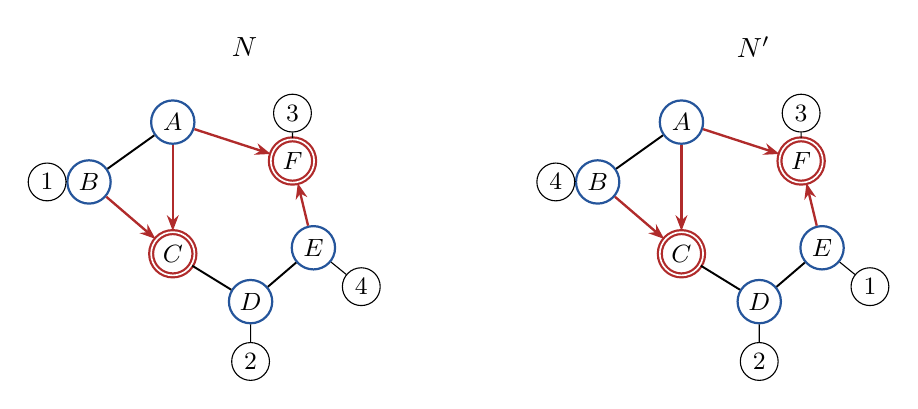
\begin{tikzpicture}[scale=.76,every node/.style={font=\small}]
\newcommand{\thetablob}[2]{%
\begin{scope}[shift={(#1,0)}]
\node[treev] (A#2) at (0,2.2) {$A$};
\node[treev] (B#2) at (-1.4,1.2) {$B$};
\node[reticv] (C#2) at (0,0) {$C$};
\node[treev] (D#2) at (1.3,-.8) {$D$};
\node[treev] (E#2) at (2.35,.1) {$E$};
\node[reticv] (F#2) at (2.0,1.55) {$F$};
\draw[reticedge] (A#2)--(C#2);
\draw[ordinary] (A#2)--(B#2);
\draw[reticedge] (B#2)--(C#2);
\draw[ordinary] (C#2)--(D#2);
\draw[ordinary] (D#2)--(E#2);
\draw[reticedge] (A#2)--(F#2);
\draw[reticedge] (E#2)--(F#2);
\end{scope}}
\thetablob{-5}{L}
\thetablob{3.5}{R}
\node[leaf] (l1) at (-7.1,1.2) {$1$};
\node[leaf] (l2) at (-3.7,-1.8) {$2$};
\node[leaf] (l3) at (-3,2.35) {$3$};
\node[leaf] (l4) at (-1.85,-.55) {$4$};
\draw (BL)--(l1); \draw (DL)--(l2); \draw (FL)--(l3); \draw (EL)--(l4);
\node[font=\bfseries] at (-3.8,3.45) {$N$};
\node[leaf] (r4) at (1.4,1.2) {$4$};
\node[leaf] (r2) at (4.8,-1.8) {$2$};
\node[leaf] (r3) at (5.5,2.35) {$3$};
\node[leaf] (r1) at (6.65,-.55) {$1$};
\draw (BR)--(r4); \draw (DR)--(r2); \draw (FR)--(r3); \draw (ER)--(r1);
\node[font=\bfseries] at (4.7,3.45) {$N'$};
\end{tikzpicture}
\caption{The standard semi-directed reductions.  Double circles are
reticulations, and arrowheads are retained only on incoming reticulation
edges.  The unique triangle is $A$--$B$--$C$.}
\label{fig:pair}
\end{figure}

After the root is suppressed, the nontrivial blob is the theta graph with
three $A$--$C$ paths
\[
A-C,\qquad A-B-C,\qquad A-F-E-D-C.
\]
Its simple cycles have lengths $3,5,6$.

In the formulas below, $x_{AC}=x_{\rho A}x_{\rho C}$ is the effective edge
created by root suppression.  The probability $\lambda_C$ selects that
$A$--$C$ parent edge and $1-\lambda_C$ selects $B\to C$; similarly,
$\lambda_F$ selects $A\to F$ and $1-\lambda_F$ selects $E\to F$.

\begin{proposition}[Combinatorial certification]\label{prop:topology}
The rooted presentations \eqref{eq:common-arcs}--\eqref{eq:Np-pendants}
are binary, level two, and tree-child.  Their standard reductions lie in
$\TCw\setminus\TCs$.  The two reductions are nonisomorphic and are not
$\Tmove$-equivalent.
\end{proposition}

\begin{proof}
The bidegrees in the displayed arc lists are $(0,2)$ at $\rho$, $(1,2)$ at
$A,B,D,E$, $(2,1)$ at $C,F$, and $(1,0)$ at the leaves.  The lists are
acyclic.  In each rooted presentation every internal vertex has a
tree-or-leaf child, so the presentation is tree-child.  The unique blob has
the three paths above and contains exactly the two reticulations $C,F$;
hence it is level two.

The displayed rooting proves weak tree-childness.  To see directly that the
mixed graph is not strongly tree-child, insert a new root on the retained arc
$B\to C$.  The internal arcs of the resulting presentation are
\[
\rho'\to B,\quad \rho'\to C,\quad B\to A,\quad A\to C,
\quad A\to F,\quad C\to D,\quad D\to E,\quad E\to F.
\]
The pendant arcs are those in \eqref{eq:N-pendants} or
\eqref{eq:Np-pendants}, respectively.  This is binary and acyclic, its root
is the LSA (the pendant leaf at $B$ and the pendant leaf at $D$ lie on
opposite root branches), and applying $\operatorname{sd}_0$ recovers the
mixed graph.  But $A$ has the two reticulations $C,F$ as its children and
hence is not tree-child.  In the terminology of Holtgrefe et
al.~\cite{HoltgrefeEtAl2026}, $A$ is an omnian.  Exhaustive rooting
enumeration finds five admissible rootings in total, only two of which are
tree-child.

In $N$, leaf $1$ is adjacent to $B$, which lies on the unique triangle.  In
$N'$, leaf $1$ is adjacent to $E$, which lies on no triangle.  This
leaf-labelled graph property is unchanged by isomorphism or by a redirection
confined to the triangle.  Thus the reductions are neither isomorphic nor
$\Tmove$-equivalent.
\end{proof}

\section{The common eight-dimensional variety}

The automorphism group of $G$ permutes its three nonzero characters.  The
zero-sum four-leaf coordinates have fifteen JC symmetry orbits, including
normalization.  We denote the fourteen nonconstant orbits by
\[
(A,B,C,D,E,F,G,H,J,K,L,M,N,O).
\]
One explicit choice of representatives is recorded in
\cref{app:certificate}.  Equality of these fourteen entries is equivalent to
equality of the complete Fourier tensor.

\begin{proposition}[Six common equations]\label{prop:invariants}
The complete displayed-tree Fourier parameterizations of both $N$ and $N'$
satisfy
\begin{align}
J-K-M+N&=0,\label{inv:1}\\
J-AH-BF+CE&=0,\label{inv:2}\\
GL-EN&=0,\label{inv:3}\\
L^2-BEH&=0,\label{inv:4}\\
BM-DL-B^2F+BCE&=0,\label{inv:5}\\
BEO-BGH-CEL+DEH&=0.\label{inv:6}
\end{align}
\end{proposition}

\begin{proof}
Each network has four displayed trees.  Substitute their split monomials
from \eqref{eq:tree-fourier}, sum with the two inheritance parameters, and
expand the six left-hand sides.  Every coefficient is zero.  The release
verifier performs this calculation from the graph encodings rather than
accepting \eqref{inv:1}--\eqref{inv:6} as input.
\end{proof}

\begin{lemma}[Implicit geometry]\label{lem:geometry}
On $BE\ne0$, equations \eqref{inv:1}--\eqref{inv:6} define an irreducible
eight-dimensional variety.  Its positive real locus is smooth.
\end{lemma}

\begin{proof}
Five equations reconstruct
\begin{align}
J&=AH+BF-CE,&
N&=GL/E,\\
M&=(DL+B^2F-BCE)/B,&
K&=J+N-M,\\
O&=(BGH+CEL-DEH)/(BE).
\label{eq:reconstruction}
\end{align}
The remaining equation is $L^2=BEH$.  The localized coordinate ring is
\[
\C[A,B,C,D,E,F,G,H,L,(BE)^{-1}]/(L^2-BEH).
\]
The defining quadratic is irreducible over the rational function field in
$A,\ldots,H$, so the ring is an integral domain of dimension eight.  Since
$\partial(L^2-BEH)/\partial H=-BE$, it is smooth on $BE\ne0$.  On the open
stochastic locus every Fourier coordinate here is a positive sum of positive
monomials, so $B,E,H,L>0$ and the physical sheet is
$L=+\sqrt{BEH}$.
\end{proof}

\section{An exact common interior point}

The two root edges are represented after root suppression by the effective
multiplier $x_{AC}=x_{\rho A}x_{\rho C}$.  The strict rooted realization
\[
x_{\rho A}=\frac23,\qquad x_{\rho C}=\frac34
\]
gives $x_{AC}=1/2$.

For $N$, set
\begin{equation}\label{eq:source-point}
\begin{gathered}
x_{D2}=\frac12,\quad x_{DE}=\frac25,\quad x_{E4}=\frac38,
\quad x_{EF}=\frac13,\quad x_{F3}=\frac12,\\
x_{CD}=\frac9{20},\quad x_{AB}=\frac35,\quad x_{B1}=\frac15,\\
x_{AC}=x_{AF}=x_{BC}=\frac12,\qquad
\lambda_C=\lambda_F=\frac12.
\end{gathered}
\end{equation}

Let $\beta$ be the smaller root of
\begin{equation}\label{eq:beta}
43337075\beta^2-36083110\beta+7336259=0,
\qquad
\frac{441}{1250}<\beta<\frac{3529}{10000}.
\end{equation}
For $N'$, set
\begin{equation}\label{eq:target-point}
\begin{gathered}
x_{D2}=\frac12,\qquad x_{DE}=\frac{171}{775},
\qquad x_{AF}=\frac{10339}{53010\beta},\\
x_{AB}=\frac{24835\beta}{20678-24835\beta},
\qquad x_{F3}=\frac{1767}{4832},
\qquad x_{CD}=\frac{9934}{12215},\\
x_{E1}=\frac{31}{190},\qquad x_{B4}=\frac{3}{20\beta},\\
x_{AC}=x_{EF}=x_{BC}=\frac12,\qquad
\lambda_C=\lambda_F=\frac12.
\end{gathered}
\end{equation}

The polynomial in \eqref{eq:beta} has opposite signs at the rational
endpoints, and the interval lies strictly below its axis of symmetry.  It
therefore isolates the smaller root.  Exact rational interval arithmetic
then proves that every multiplier in \eqref{eq:target-point} lies strictly in
$(0,1)$; no boundary or merely entrywise-positive transition matrix is used.

At these two parameter points the common orbit vector is
\begin{align}
(A,\ldots,H)&=
\left(
\frac{277}{8000},\frac3{40},\frac{67}{2400},\frac{127}{16000},
\frac{27}{5000},\frac{81}{5000},\frac{153}{160000},\frac9{500}
\right),\label{eq:first-eight}\\
(J,\ldots,O)&=
\left(
\frac{27}{16000},\frac{261}{320000},\frac{27}{10000},
\frac{27}{20000},\frac{153}{320000},\frac{183}{80000}
\right).
\label{eq:last-six}
\end{align}

To certify regularity, fix
\[
x_{AC}=x_{AF}=x_{BC}=\lambda_C=\lambda_F=\frac12
\]
for $N$ and use
\[
(P,s,Q,t,R,u,v,S)=
(x_{D2},x_{DE},x_{E4},x_{EF},x_{F3},x_{CD},x_{AB},x_{B1}).
\]
The Jacobian determinant of $(A,\ldots,H)$ is
\begin{equation}\label{eq:source-jac}
-\frac{P^3s^3Q^4tR^4u^3vS^3(s-1)^2(v-1)(v+1)^2}{16384},
\end{equation}
which is nonzero throughout the open gauge cube.

For $N'$, fix
\[
x_{AC}=x_{EF}=x_{BC}=\lambda_C=\lambda_F=\frac12
\]
and use
\[
(P',x,y,z,R',w,S',Q')=
(x_{D2},x_{DE},x_{AF},x_{AB},x_{F3},x_{CD},x_{E1},x_{B4}).
\]
The determinant is
\begin{equation}\label{eq:target-jac}
-\frac{(P')^3x^2y^2z(R')^4w^4(S')^3(Q')^4
(x-1)^2(z-1)(z+1)^3}{32768},
\end{equation}
which is also nonzero on the open cube.

\begin{proposition}[Four-leaf stochastic overlap]\label{prop:overlap}
The complete JC Fourier tensors of $N$ at \eqref{eq:source-point} and $N'$
at \eqref{eq:target-point} agree exactly.  The two stochastic model images
share a regular relatively open eight-dimensional neighborhood.
\end{proposition}

\begin{proof}
Direct displayed-tree evaluation in $\mathbb Q(\beta)$ gives
\eqref{eq:first-eight}--\eqref{eq:last-six} for both networks.  The exact
verifier checks all $256$ Fourier entries, including the forced zero
coordinates; invertibility of the Fourier transform gives equality of all
pattern probabilities.

By \cref{prop:invariants,lem:geometry}, each model lies in the same
irreducible eight-dimensional variety.  The nonzero determinants
\eqref{eq:source-jac} and \eqref{eq:target-jac} show that each image is an
eight-dimensional local submanifold at the common point.  The Zariski closure
of each parameterized image is irreducible; containment in an irreducible
eight-dimensional locus together with rank eight therefore makes both
closures equal to that locus.  Moreover, the first eight coordinates of each
stochastic image contain a neighborhood of the vector in
\eqref{eq:first-eight}.  Intersect the two neighborhoods.  Positivity forces
the same value $L=+\sqrt{BEH}$, and \eqref{eq:reconstruction} forces the other
five coordinates.  Hence the intersection contains a relative open
eight-dimensional neighborhood.
\end{proof}

\begin{corollary}\label{cor:generic-failure}
The set of parameters of $N$ admitting a realization on $N'$ contains a
nonempty Euclidean-open subset of the full parameter space.  It is not
contained in any proper algebraic subset.
\end{corollary}

\begin{proof}
The full parameterization has rank eight at the source point because the
restricted gauge map has rank eight.  The submersion theorem maps a
neighborhood of the source point onto a relative neighborhood of the common
variety.  The inverse image of the open overlap in \cref{prop:overlap} is
therefore nonempty and open.  A nonzero real polynomial cannot vanish on a
Euclidean-open parameter set.
\end{proof}

\section{Leaf substitution}

Let $P$ be a normalized positive Fourier tensor on $X\cup\{a\}$.  Replace
the leaf $a$ by a cherry with leaves $a_1,a_2$ and new pendant multipliers
$u,v\in(0,1)$.  The former pendant edge becomes the stem of the cherry.  The
new tensor is
\begin{equation}\label{eq:cherry}
\widetilde P(g_X,g_1,g_2)=
P(g_X,g_1\xor g_2)
u^{\mathbf1[g_1\ne0]}v^{\mathbf1[g_2\ne0]}.
\end{equation}

\begin{lemma}[Positive analytic inverse]\label{lem:cherry}
The map $(P,u,v)\mapsto\widetilde P$ in \eqref{eq:cherry} is a positive
real-analytic embedding.  Its inverse is real analytic on its image.
Consequently, substituting a cherry adds exactly two model dimensions and
preserves full-dimensional regular overlap.
\end{lemma}

\begin{proof}
Fix $h\in G\setminus\{0\}$.  With all characters on $X$ equal to zero,
\[
uv=\widetilde P(0,h,h),
\]
because $P(0,0)=1$.  Choose any $g_X$ with total character $h$.  Positivity of
the open JC Fourier tensor permits division, and
\[
\frac uv=
\frac{\widetilde P(g_X,h,0)}{\widetilde P(g_X,0,h)}.
\]
Thus $u$ and $v$ are recovered uniquely by the positive square root.  Every
entry of $P$ is then recovered from \eqref{eq:cherry} by division by a
positive monomial in $u,v$.  These formulas are real analytic.  Therefore
the image is analytically isomorphic to the product of the base tensor image
with $(0,1)^2$, proving the dimension and regularity assertions.
\end{proof}

\begin{proof}[Proof of \cref{thm:main}]
The case $n=4$ is \cref{prop:topology,prop:overlap}.  For each new taxon,
replace the same labelled leaf in both networks by an identically labelled
cherry.  Equation \eqref{eq:cherry} carries every common base distribution
and every common pair $(u,v)$ to the same enlarged distribution.  By
\cref{lem:cherry}, a common regular open region gains exactly two dimensions
at each step.  Starting from dimension eight gives
\[
8+2(n-4)=2n.
\]

The displayed tree-child rootings extend through each inserted cherry, so
the enlarged semi-directed topologies remain in $\TCw$.  The original
omnian at $A$ is unchanged, so they remain outside $\TCs$.  The substituted
leaf block attaches at a triangle vertex in one topology and at a
nontriangle vertex in the other.  This labelled cut-component property is
preserved by mixed-graph isomorphism and by $\Tmove$.  Thus the two enlarged
topologies remain nonisomorphic and non-$\Tmove$-equivalent.  Repeating the
construction proves the theorem for every $n\ge4$.
\end{proof}

\section{Scope and biological interpretation}

The theorem separates three notions that can otherwise be conflated.  The
two models have equal complex closures, they have a full-dimensional regular
stochastic overlap, and the exhibited parameter correspondence is strictly
inside $\Theta_0$.  We do not claim equality of the complete stochastic
images, nor that the overlap is dense in either image.

The ambiguity is also not root relocation or triangle orientation.  It
changes which labelled descendant component is attached to the triangle.
Consequently, even an exact infinite-data JC distribution cannot always
determine that attachment in the weakly tree-child level-2 class.  The
construction does not settle identifiability inside $\TCs$; that positive
classification remains outside the scope of this paper.

\section{Exact verification}\label{sec:verification}

The accompanying reproducibility package contains two implementations.  The
primary symbolic verifier derives displayed-tree Fourier parameterizations
from machine-readable rooted arc lists, checks the six identities, verifies
the two Jacobian factorizations, isolates $\beta$, proves strict positivity,
and checks all $256$ coordinates.  The independent verifier shares no graph,
Fourier, isomorphism, or number-field code with the primary implementation.
It additionally enumerates all admissible rootings and verifies the all-$n$
substitution argument at the level of exact formulas.

Every released certificate is regenerated from source.  Hashes and exact
commands are recorded in the package manifest.  Finite graph regressions for
several values of $n$ are included only as error-detection tests; the
quantified all-$n$ result is the proof of \cref{lem:cherry} and induction, not
finite enumeration.

\appendix
\section{Fourier orbit convention and algebraic data}\label{app:certificate}

Represent the nonzero elements of $G$ by $1,2,3$.  The fourteen nonconstant
JC orbits can be represented by
\begin{center}
\begin{tabular}{ccl@{\qquad}ccl}
\toprule
symbol & tuple & name & symbol & tuple & name\\
\midrule
$A$&$0011$&$r_{34}$ & $B$&$0101$&$r_{24}$\\
$C$&$0110$&$r_{23}$ & $D$&$0123$&$t_{234}$\\
$E$&$1001$&$r_{14}$ & $F$&$1010$&$r_{13}$\\
$G$&$1023$&$t_{134}$ & $H$&$1100$&$r_{12}$\\
$J$&$1111$&$u_{1111}$ & $K$&$1122$&$u_{1122}$\\
$L$&$1203$&$t_{124}$ & $M$&$1212$&$u_{1212}$\\
$N$&$1221$&$u_{1221}$ & $O$&$1230$&$t_{123}$\\
\bottomrule
\end{tabular}
\end{center}

The field is $\mathbb Q(\beta)$ with the minimal polynomial in
\eqref{eq:beta}.  Reduction uses
\[
\beta^2=\frac{36083110}{43337075}\beta-
\frac{7336259}{43337075}.
\]
The independent verifier represents every field element uniquely as
$a+b\beta$ with $a,b\in\mathbb Q$.  Equality is coefficient equality after
this reduction.  Order is never inferred from the algebraic representation;
all stochastic inequalities are proved separately using the rational
isolating interval in \eqref{eq:beta}.

\section*{Data and code availability}

The exact graph encodings, verifiers, generated certificates, source, and
deterministic reproduction command accompany this manuscript in the project
repository.  No specialized phylogenetic-classification software is needed.

\section*{Use of generative AI}

Generative AI systems assisted with exploratory algebra, implementation,
drafting, and adversarial review.  Earlier automated drafts overclaimed a
global positive classification and used an incorrect bridge-coordinate
argument; those claims were withdrawn.  The present manuscript contains only
the theorem supported by the exact, independently replayed certificates.  The
author is responsible for the statement, proof, code, and final submission.

\begin{thebibliography}{99}

\bibitem{Ardiyansyah2021}
M. Ardiyansyah,
\emph{Distinguishing Level-2 Phylogenetic Networks Using Phylogenetic
Invariants}, arXiv:2104.12479 (2021).

\bibitem{BritsEtAl2026}
J. Brits, N. Holtgrefe, L. van Iersel, and S. Martin,
\emph{On Tree--Network Distinguishability and Full Identifiability of
Phylogenetic Networks}, arXiv:2607.12919v2 (2026).

\bibitem{CurrieEtAl2026}
B. Currie, A. K. Englander, J. A. Esparza-Lozano, E. Gross, M. Hill,
C. Long, D. Olds, K. O'Connor, U. Ranasinghe, and C. Sum,
\emph{Semialgebraic Conditions for Identifying Triangles in Phylogenetic
Networks}, arXiv:2606.26673 (2026).

\bibitem{EnglanderEtAl2026}
A. K. Englander, M. Frohn, E. Gross, N. Holtgrefe, L. van Iersel,
M. Jones, and S. Sullivant,
\emph{Identifiability of Phylogenetic Level-2 Networks under the
Jukes--Cantor Model}, bioRxiv 2025.04.18.649493, version 4 (2026),
\url{https://doi.org/10.1101/2025.04.18.649493}.

\bibitem{EvansSpeed1993}
S. N. Evans and T. P. Speed,
\emph{Invariants of Some Probability Models Used in Phylogenetic Inference},
Ann. Statist. 21 (1993), 355--377.

\bibitem{HoltgrefeEtAl2026}
N. Holtgrefe, K. T. Huber, L. van Iersel, M. Jones, and V. Moulton,
\emph{Characterizing Semi-Directed Phylogenetic Networks and Their
Multi-Rootable Variants}, Theory Biosci. 145 (2026), article 4,
\url{https://doi.org/10.1007/s12064-025-00453-8}.

\bibitem{SturmfelsSullivant2005}
B. Sturmfels and S. Sullivant,
\emph{Toric Ideals of Phylogenetic Invariants},
J. Comput. Biol. 12 (2005), 204--228.

\bibitem{Sullivant2026}
S. Sullivant,
\emph{Phylogenetic Network Models as Graphical Models},
arXiv:2507.23056v2 (2026).

\end{thebibliography}

\end{document}
